% Appendix A

\chapter{Tabellen, Diagramme und Befragungsergebnisse}
\label{Tabellen_Modelle_Diagramme}

\section{Stakeholderanalyse}

\begin{table}[H]
	\centering
	\caption[Stakeholderanalyse]{Stakeholder für E-Mails in Unternehmen}
		\vspace{1.0em}	
    \begin{tabular}{|l|l|l|l|}
    \rowcolor{red!25}
    \hline
    \textbf{Bezeichnung}                   & \textbf{Beziehung} & \textbf{Objektbereich}                                             & \textbf{Prio} \\ \hline
    Absender              & Anrecht            & Unlimitierter Versand von E-Mails                                  & 1                  \\ \cline{2-4} 
                                           & Interesse          & Beantwortung von E-Mails                                           & 1                  \\ \cline{2-4} 
                                           & Interesse          & Voraussichtliche Antwortzeit                                       & 1                  \\ \hline
    Empfänger             & Anrecht            & Erreichbarkeit                                                     & 1                  \\ \cline{2-4} 
                                           & Anrecht            & Eigene Zeiteinteilung bei Triage                                   & 2                  \\ \cline{2-4} 
                                           & Interesse          & Strukturierte E-Mails                                              & 2                  \\ \cline{2-4} 
                                           & Interesse          & Benachrichtigung bei neuen E-Mails                                   & 1                  \\ \cline{2-4} 
                                           & Interesse          & Einfach erkennbare Priorität von E-Mails                           & 2                  \\ \hline
    Management            & Anspruch           & Produktivität von Mitarbeitern trotz E-Mails                       & 2                  \\ \cline{2-4} 
                                           & Anspruch           & Erreichbarkeit der Mitarbeiter                                     & 1                  \\ \hline
    ISP                                    & Anteil             & Anteil an externer Infrastruktur von E-Mails         & 2                  \\ \hline
    Administratoren & Anteil             & Interne Infrastruktur                                              & 1                  \\ \cline{2-4} 
                                           & Anteil             & Schutzmaßnahmen vor Spam und Angriffen via E-Mail                  & 2                  \\ \hline
    Betriebsräte                           & Interesse          & Interesse an sozialen Auswirkungen auf Empfänger & 3                  \\ \hline
    \end{tabular}
	\label{tab:stakeholderanalyse}
\end{table}
% ------------------------------------------------------


\section{Ergebnisse der Befragung zu Bezahl- und Tokensystemen}

\begin{table}[H]
\centering
	\caption[Rohdaten der Befragung]{Rohdaten der Befragung zu Bezahl- und Tokensystemen}
\begin{tabular}{lllll}
\rowcolor{red!25}
\hline
\multicolumn{1}{|l|}{\textbf{Nr.}} & \multicolumn{1}{l|}{\textbf{Geschlecht}} & \multicolumn{1}{l|}{\textbf{Alter}} & \multicolumn{1}{l|}{\textbf{Jahresbruttoeinkommen}} & \multicolumn{1}{l|}{\textbf{Auswahl}} \\ \hline
1                                  & w                                        & 61                                  & 21.402,36 €                             & Echtgeld                              \\
2                                  & m                                        & 53                                  & 51.985,88 €                             & Echtgeld                              \\
3                                  & m                                        & 44                                  & 49.219,10 €                             & Keine Zahlung                         \\
4                                  & m                                        & 32                                  & 29.004,00 €                             & Echtgeld                              \\
5                                  & k.A.                                     & 57                                  & 78.000,00 €                             & Token                                 \\
6                                  & w                                        & 42                                  & 27.333,59 €                             & Token                                 \\
7                                  & w                                        & 45                                  & 40.008,00 €                             & Echtgeld                              \\
8                                  & w                                        & 35                                  & 42.000,00 €                             & Echtgeld                              \\
9                                  & w                                        & 23                                  & 21.600,00 €                             & Echtgeld                              \\
10                                 & m                                        & 35                                  & 43.299,54 €                             & Echtgeld                              \\
11                                 & w                                        & 31                                  & 36.848,84 €                             & Token                                 \\
12                                 & m                                        & 48                                  & 58.847,15 €                             & Token                                 \\
13                                 & m                                        & 23                                  & 12.960,00 €                             & Echtgeld                              \\
14                                 & w                                        & 49                                  & 10.644,00 €                             & Keine Zahlung                         \\
15                                 & m                                        & 28                                  & 34.524,00 €                             & Echtgeld                              \\
16                                 & w                                        & 23                                  & 13.310,97 €                             & Echtgeld                              \\
17                                 & m                                        & 24                                  & 15.598,80 €                             & Token                                 \\
18                                 & w                                        & 52                                  & 55.115,06 €                             & Echtgeld                              \\
19                                 & k.A.                                     & 36                                  & 46.706,47 €                             & Echtgeld                              \\
20                                 & m                                        & 52                                  & 105.000,00 €                            & Echtgeld                              \\
21                                 & w                                        & 27                                  & 31.468,19 €                             & Keine Zahlung                         \\
22                                 & w                                        & 24                                  & 26.578,84 €                             & Echtgeld                              \\
23                                 & m                                        & 22                                  & 12.960,00 €                             & Echtgeld                              \\
24                                 & w                                        & 58                                  & 73.152,00 €                             & Echtgeld                              \\
25                                 & m                                        & 53                                  & 59.020,00 €                             & Echtgeld                              \\
26                                 & k.A.                                     & 27                                  & 8.028,00 €                              & Keine Zahlung                         \\
27                                 & w                                        & 48                                  & 39.000,00 €                             & Echtgeld                              \\
28                                 & w                                        & 28                                  & 25.849,54 €                             & Token                                 \\
29                                 & m                                        & 21                                  & 15.792,00 €                             & Token                                 \\
30                                 & k.A.                                     & 20                                  & 2.628,00 €                              & Keine Zahlung                         \\
31                                 & m                                        & 33                                  & 8.016,51 €                              & Echtgeld                              \\
32                                 & w                                        & 20                                  & 19.245,15 €                             & Token                                 \\
33                                 & m                                        & 49                                  & 50.572,81 €                             & Echtgeld                              \\
34                                 & m                                        & 18                                  & 900,00 €                                & Keine Zahlung                         \\
35                                 & w                                        & 54                                  & 46.000,00 €                             & Echtgeld                              \\
36                                 & w                                        & 46                                  & 38.959,55 €                             & Echtgeld                              \\
37                                 & m                                        & 62                                  & 65.000,00 €                             & Echtgeld                              \\
38                                 & w                                        & 34                                  & 39.708,00 €                             & Echtgeld                              \\
39                                 & m                                        & 22                                  & 12.960,00 €                             & Token                                
\end{tabular}
\label{tab:rohdaten}
\end{table}

% ------------------------------------------------------
\subsection{Ergebnisse der Befragung nach Geschlecht}

\begin{figure}[H]
\centering
\caption[Ergebnisse der Befragung nach Geschlecht]{Ergebnisse der Befragung nach Geschlecht}
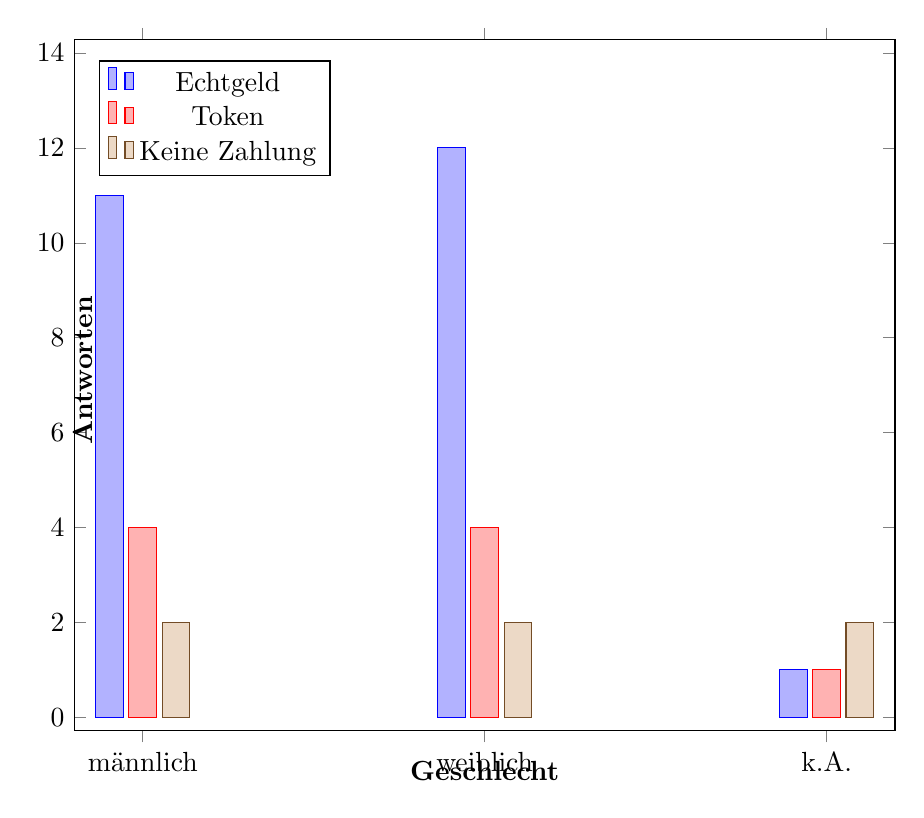
\begin{tikzpicture}
    \begin{axis}[
        ybar,
        ymin=0,ymax=14,
        x label style={at={(axis description cs:0.5,-0.03)},anchor=north},
        y label style={at={(axis description cs:0.01,0.4)},anchor=west},
        ylabel= \textbf{Antworten},
        xlabel= \textbf{Geschlecht},
        enlarge x limits  = 0.1,
        enlarge y limits  = 0.02,
        symbolic x coords={männlich,weiblich,k.A.},
        xtick=data,
        width=0.99\textwidth,
        legend pos=north west
    ]
    \addplot coordinates
    {(männlich, 11) (weiblich, 12) (k.A., 1)};
    \addplot coordinates
    {(männlich, 4) (weiblich, 4) (k.A., 1)};
    \addplot coordinates
    {(männlich, 2) (weiblich, 2) (k.A., 2)};
    \legend{Echtgeld, Token, Keine Zahlung}
    \end{axis}
\end{tikzpicture}
\label{fig:Ergebnisse_der_Befragung_nach_Geschlecht}
\end{figure}


% ------------------------------------------------------
\subsection{Ergebnisse der Befragung nach Alter}

\begin{figure}[H]
\centering
\caption[Ergebnisse der Befragung nach Alter]{Ergebnisse der Befragung nach Alter}
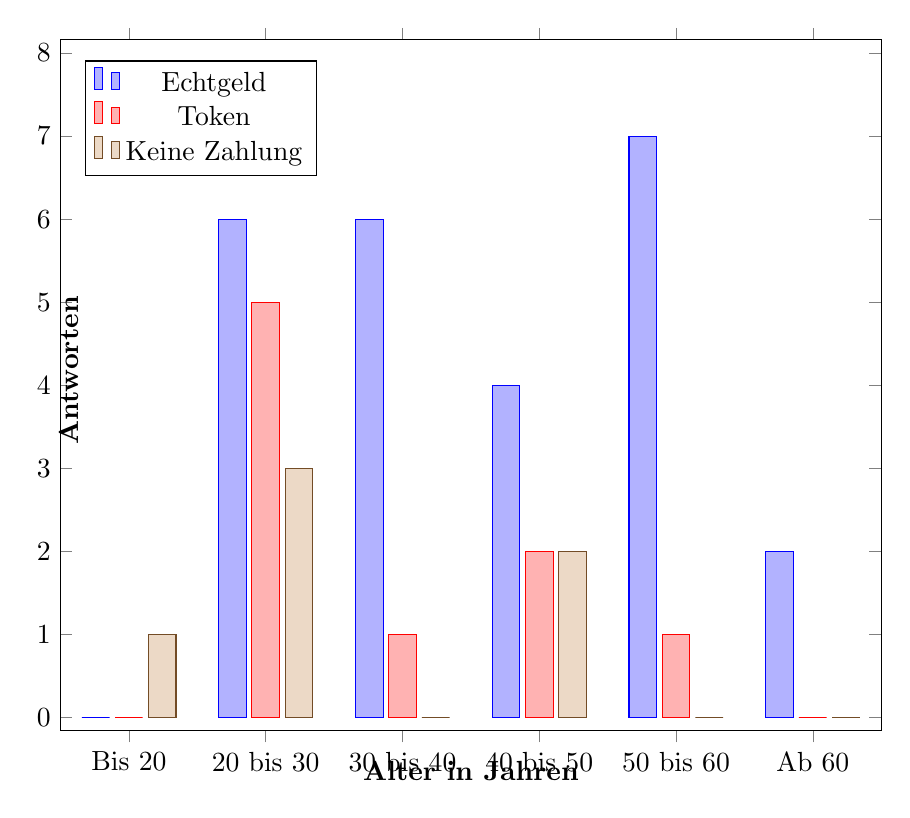
\begin{tikzpicture}
    \begin{axis}[
        ybar,
        ymin=0,ymax=8,
        x label style={at={(axis description cs:0.5,-0.03)},anchor=north},
        y label style={at={(axis description cs:0.01,0.4)},anchor=west},
        ylabel= \textbf{Antworten},
        xlabel= \textbf{Alter in Jahren},
        enlarge x limits  = 0.1,
        enlarge y limits  = 0.02,
        symbolic x coords={Bis 20,20 bis 30,30 bis 40,40 bis 50,50 bis 60,Ab 60},
        xtick=data,
        width=0.99\textwidth,
        legend pos=north west
    ]
    \addplot coordinates
    {(Bis 20, 0) (20 bis 30, 6) (30 bis 40, 6) (40 bis 50, 4) (50 bis 60, 7) (Ab 60, 2)};
    \addplot coordinates
    {(Bis 20, 0) (20 bis 30, 5) (30 bis 40, 1) (40 bis 50, 2) (50 bis 60, 1) (Ab 60, 0)};
    \addplot coordinates
    {(Bis 20, 1) (20 bis 30, 3) (30 bis 40, 0) (40 bis 50, 2) (50 bis 60, 0) (Ab 60, 0)};
    \legend{Echtgeld, Token, Keine Zahlung}
    \end{axis}
\end{tikzpicture}
\label{fig:Ergebnisse_der_Befragung_nach_Alter}
\end{figure}



\newpage
% ------------------------------------------------------
\section{Notizen und Antworten der Nutzerevaluation}
\label{Notizen_und_Antworten_der_Nutzerevaluation}

\subsection{Absender 1}
Alter: 36 \\
Beruf: Chemieingenieur \\
Geschlecht: männlich \\
Jahresbruttoeinkommen: 59.000€

\subsubsection*{Notizen während der in vivo Evaluation}
\begin{itemize}
    \item Verwirrt, ob die E-Mail Adresse richtig erfasst wurde, da sie bei \texttt{/capacities} nicht mehr angezeigt wird, sondern nur der Name.
    \item Es ist nicht klar was das Minimum und Maximum an Zahlungen ist, Beschreibungstexte wären hilfreich.
    \item E-Mail Adresse wird bei \texttt{/priority/new} nicht übernommen.
    \item Es gibt keine Möglichkeit zurück zum Anfang zu navigieren ohne die Browser-Navigation.
    \item Nutzung des Gegenwertheaders ist direkt verstanden worden.
\end{itemize}

\subsubsection*{Beantwortung der Fragen}
\begin{enumerate}
\item E-Mails werden effektiver, allerdings leidet die Effizienz, da die Priorisierung den Versandprozess erweitert und verlängert. Ist man an den Prozess gewöhnt, kann die Effizienz sich jedoch wieder verbessern.
\item Ja, insbesondere da die Einsicht in das Aufkommen optional ist kann ich selbst entscheiden, ob ich das Aufkommen sehen will. Außerdem habe ich so eine bessere Grundlage zur Entscheidung, ob ich eine E-Mail priorisieren will.
\setcounter{enumi}{4}
\item Generell unterstützt das System in der Bearbeitung von E-Mails, allerdings liegt die Priorisierung ausschließlich in den Händen der Absender. Dadurch kann man sich vordrängeln, wenn man genug Geld hat, unabhängig davon wie wichtig die E-Mail wirklich ist.
\item Das System sollte einem deutlicher aufzeigen wo man sich befindet und wie man navigieren kann. Außerdem sollte man nach der Priorisierung informiert werden, falls sich das Bearbeitungsdatum verschiebt oder man überboten wird.
\end{enumerate}

\subsection{Absender 2}
Alter: 24 \\
Beruf: Rechtsanwaltsfachangestellte \\
Geschlecht: weiblich \\
Jahresbruttoeinkommen: 21.600€

\subsubsection*{Notizen während der in vivo Evaluation}
\begin{itemize}
    \item Unterschied zwischen Priorität und Aufkommen ist nicht ganz klar.
    \item Das System von Priorisierung wird daraufhin auf Anhieb verstanden.
    \item Es fehlt eine genaue Anleitung wie der Gegenwert-Header genutzt werden soll, Prinzip wurde jedoch verstanden.
\end{itemize}

\subsubsection*{Beantwortung der Fragen}
\begin{enumerate}
\item Ja, denn man kann je nach Dringlichkeit seine E-Mail vorne einordnen oder warten, bis man dran ist.
\item Ja, die Transparenz ist ein großer Vorteil und sorgt dafür, dass man ein besseres Gefühl für den Empfänger bekommt.
\setcounter{enumi}{4}
\item Es löst das generelle Problem nicht, aber es hilft den Prozess zu optimieren.
\item Es sollten mehr erklärende Texte hinzugefügt werden.
\end{enumerate}

\subsection{Empfänger 1}
Alter: 21 \\
Beruf: Student \\
Geschlecht: männlich \\
Jahresbruttoeinkommen: 15.464€

\subsubsection*{Notizen während der in vivo Evaluation}
\begin{itemize}
    \item Das System und die Funktionsweise werden direkt verstanden.
    \item Der soziale Aspekt des Systems im Generellen wird hinterfragt.
    \item Ausnahmeregeln könnten den sozialen Aspekt lösen, aber dafür muss der Empfänger wissen, welche Personen eine E-Mail priorisieren wollten und es sich nicht leisten konnten.
\end{itemize}

\subsubsection*{Beantwortung der Fragen}
\begin{enumerate}
\setcounter{enumi}{2}
\item Ja, insbesondere da ich mit Ausnahmeregeln meine bisherigen wichtigen Absender weiter priorisieren kann.
\item Ja, sie ergänzen die automatische Triage gut, wobei es zu wenig Felder gibt, nach denen ich filtern kann.
\item Dadurch, dass man die Verantwortung der Priorisierung an die Absender abgibt, kann man dafür nicht in Rechenschaft gezogen werden. Das löst den Overload nicht, hilft aber bei der Bewältigung.
\item Es sollte eine Möglichkeit geben sozial schwache Personen gezielt bei der Priorisierung zu unterstützen/zu subventionieren, damit sie im Wettbewerb und schnelle Beantwortung mithalten können.
\end{enumerate}

\subsection{Empfänger 2}
Alter: 47 \\
Beruf: Projektmanagerin (selbstständig) \\
Geschlecht: weiblich \\
Jahresbruttoeinkommen: 66.234€

\subsubsection*{Notizen während der in vivo Evaluation}
\begin{itemize}
    \item Das System und die Funktionsweise werden direkt verstanden.
    \item Frage: Muss der Empfänger wissen wie viel gezahlt wurde? Das könnte Druck auslösen, wenn man darüber nachdenkt als Empfänger. 
    \item Gibt es eine Absicherung, dass keine Nachrichten ignoriert werden, die eigentlich sehr wichtig (aber ohne Zahlung versehen) sind?
    \item Obige Frage wird nach Vorstellung der Ausnahmeregeln zurückgezogen.
\end{itemize}

\subsubsection*{Beantwortung der Fragen}
\begin{enumerate}
\setcounter{enumi}{2}
\item Ja, denn die Triage wird zumindest teilweise abgenommen. Trotzdem sehe ich mir die Betreffe der Nachrichten an, damit nichts untergeht.
\item Ja, diese Funktion ist sehr relevant, wie bereits erwähnt. Allerdings ist kann es zu Beginn sehr zeitaufwändig sein passende Regeln zu definieren.
\item Wenn andere meinen Overload im Vorhinein sehen und wissen auf welche Antwortzeiten sie sich einstellen müssen, wirkt das dem Stress der Bearbeitung entgegen und erzeugt unter Umständen Rücksicht bei Absendern. Sobald diese Rücksicht etabliert ist, wird auch Overload gelöst.
\item Die Triage sollte sich nur in bestimmten Intervallen (1 bis 2 Stunden) ändern können. Ansonsten ändert sich die Reihenfolge der E-Mails mit jeder neu versendeten Mail, was dazu führt, dass man unter Umständen E-Mails bearbeitet, die ihre Priorität bereits verloren haben.
\end{enumerate}

% ------------------------------------------------------
\newpage

\section{Ordnerstruktur der Anwendung}
\label{Ordnerstruktur_der_Anwendung}

\begin{itemize}
    \item \texttt{.github/}
    \begin{itemize}
        \item \texttt{workflows/}
    \end{itemize}
    \item \texttt{app/}
    \begin{itemize}
        \item \texttt{assets/}
        \item \texttt{channels/}
        \item \texttt{controllers/}
        \item \texttt{helpers/}
        \item \texttt{javascript/}
        \item \texttt{jobs/}
        \item \texttt{mailers/}
        \item \texttt{models/}
        \item \texttt{services/}
        \item \texttt{views/}
    \end{itemize}
    \item \texttt{bin/}
    \item \texttt{config/}
    \begin{itemize}
        \item \texttt{environments/}
        \item \texttt{initializers/}
        \item \texttt{locales/}
    \end{itemize}
    \item \texttt{db/}
    \begin{itemize}
        \item \texttt{migrate/}
    \end{itemize}
    \item \texttt{lib/}
    \begin{itemize}
        \item \texttt{assets/}
        \item \texttt{tasks/}
    \end{itemize}
    \item \texttt{public/}
    \item \texttt{storage/}
    \item \texttt{test/}
    \begin{itemize}
        \item \texttt{channels/}
        \item \texttt{controllers/}
        \item \texttt{fixtures/}
        \item \texttt{helpers/}
        \item \texttt{jobs/}
        \item \texttt{mailers/}
        \item \texttt{models/}
        \item \texttt{system/}
    \end{itemize}
    \item \texttt{vendor/}
    \begin{itemize}
        \item \texttt{javascript/}
    \end{itemize}
\end{itemize}

% ------------------------------------------------------
\newpage

\section{Routenstruktur der Anwendung}
\label{Routenstruktur_der_Anwendung}

\begin{itemize}
    \item \texttt{overview}: Startseite
    \item \texttt{sender}
    \begin{itemize}
        \item \texttt{overview}
        \begin{itemize}
            \item \texttt{index}: Landingpage Absender
        \end{itemize}
        \item \texttt{capacities}
        \begin{itemize}
            \item \texttt{index}: Auflistung des aktuellen Aufkommens
        \end{itemize}
        \item \texttt{priorities}
        \begin{itemize}
            \item \texttt{index}: Auflistung der bisher priorisierten E-Mails
            \item \texttt{new}: Formular zum Priorisieren einer E-Mail
            \item \texttt{show}: Anzeigen der UUID nach Priorisieren einer E-Mail
        \end{itemize}
    \end{itemize}
    \item \texttt{recipient}
    \begin{itemize}
        \item \texttt{sessions}
         \begin{itemize}
            \item \texttt{new}: Einloggen
            \item \texttt{destroy}: Ausloggen
        \end{itemize}
        \item \texttt{recipients}
        \begin{itemize}
            \item \texttt{new}: Formular zum Erstellen eines neuen Accounts  
            \item \texttt{edit}: Anpassen der Regeln und Bearbeitungsleistung
        \end{itemize}
        \item \texttt{rules}
        \begin{itemize}
            \item \texttt{index}: Auflistung aller Regeln
            \item \texttt{new}: Formular zum Erstellen einer neuen Regel
            \item \texttt{edit}: Formular zum Ändern einer Regeln
            \item \texttt{destroy}: Löschen einer Regel 
        \end{itemize}
        \item \texttt{inbox}
        \begin{itemize}
            \item \texttt{inbox}: Anzeige der E-Mails innerhalb der Triage
        \end{itemize}
        \item \texttt{messages}
        \begin{itemize}
            \item \texttt{show}: Anzeige einer einzelnen E-Mail  
            \item \texttt{destroy}: Erledigen einer E-Mail
        \end{itemize}
    \end{itemize}
\end{itemize}